\documentclass[epsfig,11pt]{article}
\usepackage[english]{babel} % Using babel for hyphenation
\usepackage{lmodern} % Changing the font
\usepackage[utf8]{inputenc}
\usepackage[T1]{fontenc}

\usepackage{listings}
\usepackage{amssymb}
\usepackage{graphicx}
\usepackage{amsmath}
\usepackage{epsfig}
\usepackage[parfill]{parskip} % Removes indents
\usepackage{color}
\usepackage{framed}
\usepackage{vmargin}
\usepackage{wrapfig}
\setpapersize{A4}

\definecolor{red}{rgb}{1,0.1,0}

\newcommand{\inr}[1]{ \Big \langle #1 \Big \rangle}
\newcommand\pd[2][]{\ensuremath{\frac{\partial#1}{\partial#2}}} 

\title{Applications of finite element methods in biomechanics}
\author{Krister Stræte Karlsen}

% Define colors for python code 
\definecolor{Code}{rgb}{0,0,0}
\definecolor{Decorators}{rgb}{0.5,0.5,0.5}
\definecolor{Numbers}{rgb}{0.5,0,0}
\definecolor{MatchingBrackets}{rgb}{0.25,0.5,0.5}
\definecolor{Keywords}{rgb}{0,0,1}
\definecolor{self}{rgb}{0,0,0}
\definecolor{Strings}{rgb}{0,0.63,0}
\definecolor{Comments}{rgb}{0,0.63,1}
\definecolor{Backquotes}{rgb}{0,0,0}
\definecolor{Classname}{rgb}{0,0,0}
\definecolor{FunctionName}{rgb}{0,0,0}
\definecolor{Operators}{rgb}{0,0,0}
\definecolor{Background}{rgb}{0.98,0.98,0.98}

\lstnewenvironment{python}[1][]{
\lstset{
numbers=left,
breaklines=true
numberstyle=\footnotesize,
numbersep=1em,
xleftmargin=1em,
framextopmargin=2em,
framexbottommargin=2em,
showspaces=false,
showtabs=false,
showstringspaces=false,
frame=l,
tabsize=4,
% Basic
basicstyle=\ttfamily ,
backgroundcolor=\color{Background},
language=Python,
% Comments
commentstyle=\color{Comments}\slshape,
% Strings
stringstyle=\color{Strings},
morecomment=[s][\color{Strings}]{"""}{"""},
morecomment=[s][\color{Strings}]{'''}{'''},
% keywords
morekeywords={import,from,class,def,for,while,if,is,in,elif,else,not,and,or,print,break,continue,return,True,False,None,access,as,,del,except,exec,finally,global,import,lambda,pass,print,raise,try,assert},
keywordstyle={\color{Keywords}\bfseries},
% additional keywords
morekeywords={[2]@invariant},
keywordstyle={[2]\color{Decorators}\slshape},
emph={self},
emphstyle={\color{self}\slshape},
%
}}{}

\begin{document}

\maketitle

All data belonging to this chapter can be found in: \\
{\color{Strings} \texttt{https://github.com/krikarls/fun-with-fem.git} }

\section{Blood flow in zebrafish}

Since the 1960s, the zebrafish has become increasingly important to scientific research. It has many characteristics that make it a valuable model for studying human genetics and disease. It was the first vertebrate to be cloned and is particularly notable for its regenerative abilities. Zebrafish have a similar genetic structure to humans. They share 70 per cent of genes with us and they are cheaper to maintain than mice. The zebrafish adult is about 2.5 cm to 4 cm long. 

\begin{wrapfigure}{r}{0.5\textwidth}
  \begin{center}
    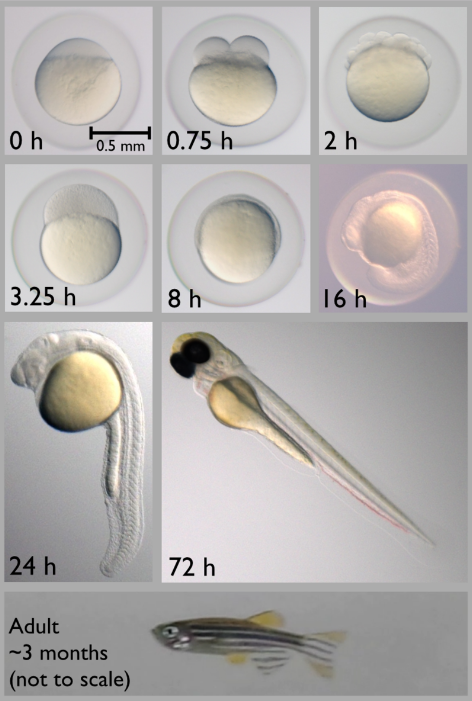
\includegraphics[width=0.4\textwidth]{zebrafish.png}
  \end{center}
  \caption{Stages of zebrafish development.}
      \label{fig:zebrafisk_development}
\end{wrapfigure}

To study the effect of different drugs being able to model the blood flow is important. For instance, if the drug actually never reaches the infected cells a potentially effective drug might be considered ineffective on wrong ground. Due to ethical reasons all experiments on zebrafish must be done at an very early stage of its development. Se Figure \ref{fig:zebrafisk_development}.

\subsection{Measurement of blood velocities in zebrafish}

The small and transparent zebrafish embryo provides an ideal animal model to get high-resolution imaging of vessels. In \cite{fieramonti2015quantitative} a method referred to as \emph{optical vector field tomography} is used to map in 3D the velocity of blood cells in the zebrafish vascular network. Some of the results in \cite{fieramonti2015quantitative} are featured in Figure \ref{fig:blood_velocity}.

\begin{figure}[h!] 
\begin{center}
  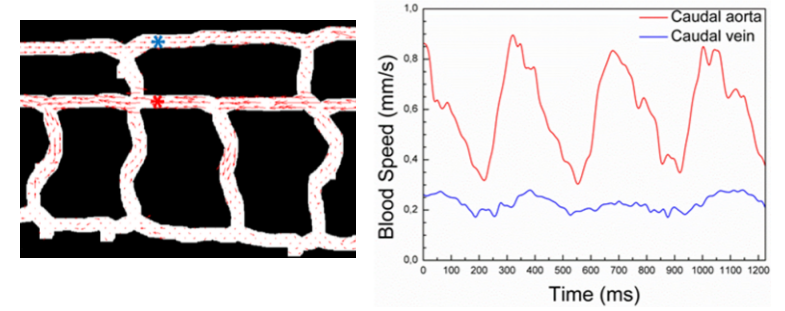
\includegraphics[scale=0.5]{blood_velocities.png}
  \end{center}
  \caption{Some of results from \cite{fieramonti2015quantitative}.}
        \label{fig:blood_velocity}
\end{figure}

\textbf{Suggested project:} Very little is known about the pressure gradients driving the blood flows in zebrafish. With knowledge of the velocities from \cite{fieramonti2015quantitative}, a mesh of geometry and a suitable model for the blood flow, do numerical experiments to find approximate values of the pressure gradients in zebrafish.

\subsection{Generating mesh from original MRI images}

{\color{red} Kent: Kan du si noe om hva slags bilder dette er?}

Starting from \texttt{original\_zebrafish.vti} a finite element method mesh can be created using a software called \emph{The Vascular Modeling Toolkit(VMTK)}. VMTK is a collection of libraries and tools for 3D reconstruction, geometric analysis, mesh generation and surface data analysis for image-based modeling of blood vessels. To install the development version of VMTK(this is strongly suggested) go through the follwing steps: 

 \begin{figure}[h!] 
\begin{center}
  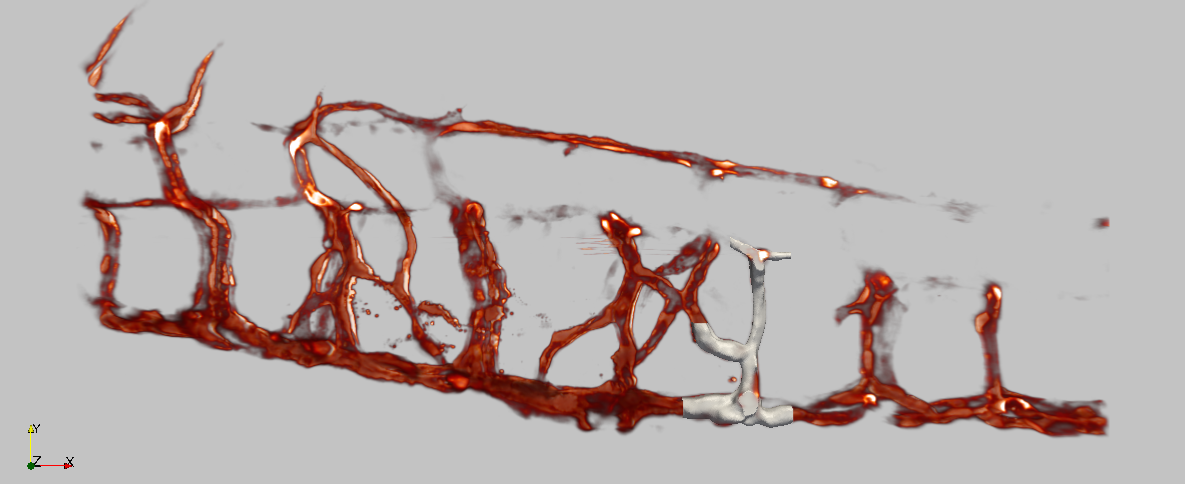
\includegraphics[scale=0.3]{overview2.png}
  \end{center}
  \caption{The circulatory system of a zebrafish where a small part is meshed.}
\label{fig:circulatory_system}
\end{figure}

\quad 1) Clone the git repository: {\color{Strings} \texttt{https://github.com/vmtk/vmtk.git}}

\quad 2) Create a build directory and cd into it

\quad 3) Run \texttt{cmake ../vmtk} with a path to vmtk source tree

\quad 4) Start the compiler in your build directory by running \texttt{make}

Next, the steps needed to create a mesh from the image-file is outlined. The reader is advised to experiment with the different parameteres used in the scripts, and the parameters suggested here should serve only as a staring point. For more information see {\color{Strings}\texttt{http://www.vmtk.org/tutorials/}}.

\vspace{0.5cm}

1) Select a volume of interest
\begin{framed}       
    \texttt{vmtkimagevoiselector -ifile original.vti -ofile voi.vti}
\end{framed}
2) Segmentation (this is tricky and very time consuming)
\begin{framed}       
    \texttt{vmtklevelsetsegmentation -ifile voi.vti -ofile levelsets.vti}
\end{framed}
3) Create surface file
\begin{framed}       
    \texttt{vmtkmarchingcubes -ifile levelsets.vti -ofile surf.vtp}
\end{framed}
4) Smoothing of surface
\begin{framed}       
    \texttt{vmtksurfacesmoothing -ifile surf.vtp -passband 0.1 -iterations 30 -ofile sm\_surf.vtp}
\end{framed}

\begin{figure}[h!] 
\begin{center}
  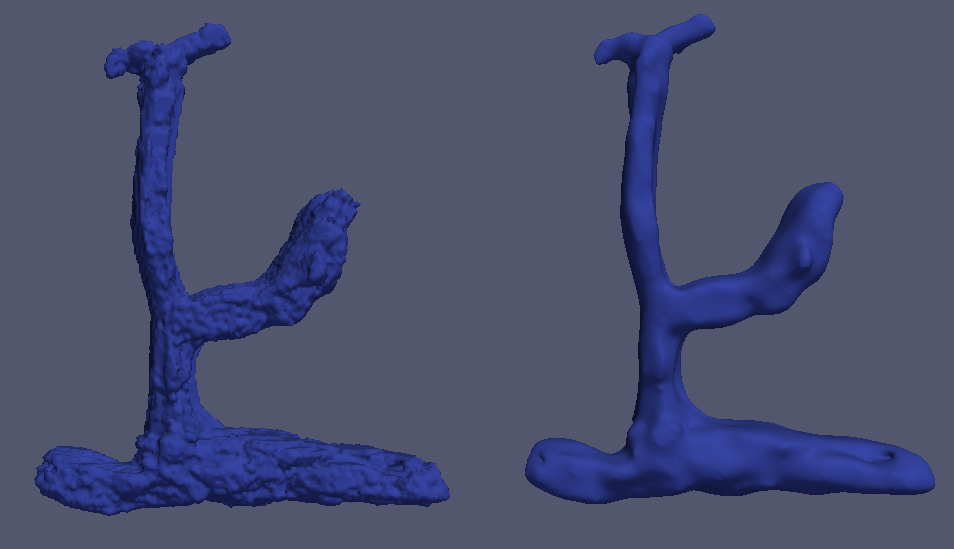
\includegraphics[scale=0.3]{smoothing.png}
  \end{center}
  \caption{Surface before and after smoothing, i.e. \texttt{surf.vtp} and \texttt{sm\_surf.vtp}.}
  \label{fig:smoothing}
\end{figure}

5) Clip surface to create openings
\begin{framed}       
    \texttt{vmtksurfaceclipper -ifile sm\_surf.vtp -ofile cl\_surface.vtp}
\end{framed}

Two of the openings in \texttt{cl\_surface.vtp} should not be there. They appear because parts of the vessels lie outside the original image. These must be capped. For the capping to be successful the openings should be clipped first so that the edges are straight.

6) Cap openings 
\begin{framed}    
\texttt{vmtksurfacecapper -ifile cl\_surf.vtp -ofile cap\_surf.vtp}
\end{framed}
7) Remesh. This is usually needed after clipping and capping, see Figure \ref{fig:remesh}. 
\begin{framed}    
\texttt{vmtksurfaceremeshing -ifile cap\_surf.vtp -ofile remeshed\_surf.stl}
\end{framed}

\begin{figure}[h!] 
\begin{center}
  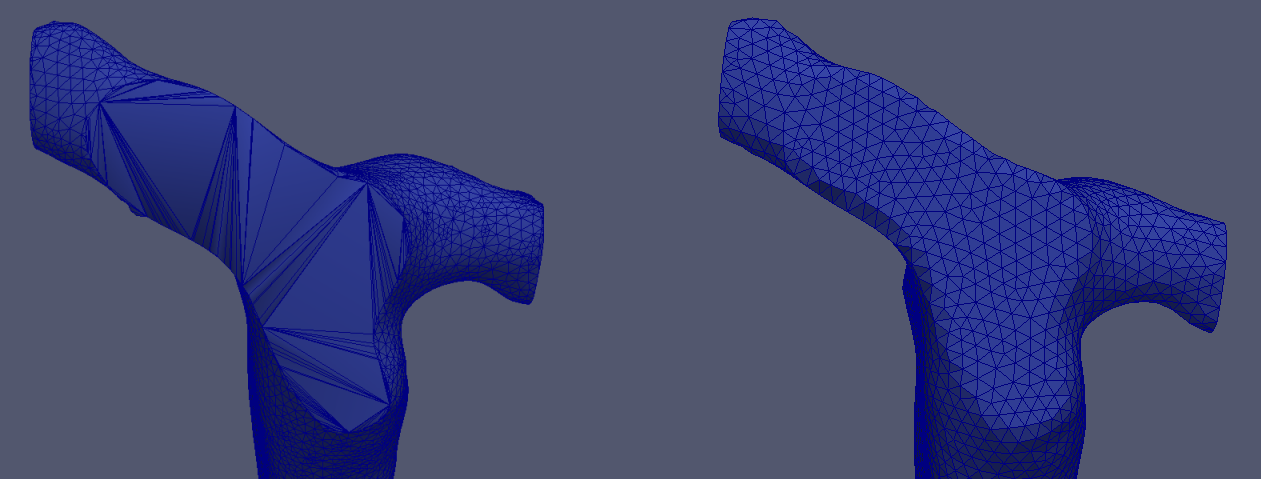
\includegraphics[scale=0.3]{remsh.png}
  \end{center}
  \caption{Before and after remeshing}
    \label{fig:remesh}
\end{figure}

In order to successfully generate a volumemesh using VMTK the surface has to perfect and there's a good chance that remeshing was not sufficient. Luckily there are other software with excellent cleaning filters to take care of the job. For example the open source software \emph{MeshLab}, available in ubuntu repository. 

Next MeshLabs clean filter called \emph{remove isolated pieces(wrt diameter) } is used to create \texttt{cleaned\_surf.stl}. This is now a perfectly good surface ready for mesh generation!

8) Generate mesh
\begin{framed}       
    \texttt{vmtkmeshgenerator -ifile cl\_surf.vtp -ofile zebramesh.vtu -edgelength 1.0}
\end{framed}

You'll see that for this mesh \texttt{edgelength 1.0} gives a very fine mesh that calls for the need for a computer cluster. So some bigger edgelength is recommended.

9) Convert to dolfin-format
\begin{framed}       
    \texttt{vmtkmeshwriter -ifile zebramesh.vtu -entityidsarray CellEntityIds -ofile zebra\_mesh.xml}
\end{framed}

The mesh can now be imported with FEniCS and blood can start flowing. 

\begin{python}
from fenics import *
mesh = Mesh('mesh.xml')
plot(mesh,interactive=True)
\end{python}

\newpage

\textbf{Marking openings in FEniCS}

Subdomains of the inlets and outlets need to be made and for complex geometries that might not be trivial. If the surface was clipped in a clever way, the job can still be pretty easy. A clever way to clip is placing the openings orthogonal to the coordinate axes(unless you love finding equations of planes).

1) Open the final surface file in ParaView.

2) Select the points around one opening and use \emph{extract selection}.

3) The range of the points(\emph{"bounds"}) can now be found and marked in FEniCS.

\textbf{Example:}

\begin{figure}[h!] 
\begin{center}
  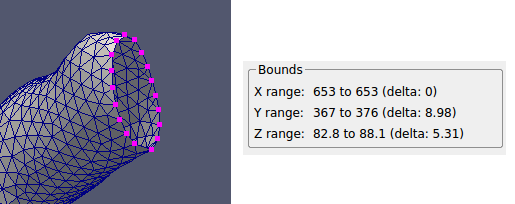
\includegraphics[scale=0.5]{marking.png}
  \end{center}
  \caption{Marking of points and finding their range in ParaView.}
      \label{fig:marking_paraview}
\end{figure}

From Figure \ref{fig:marking_paraview} we can see that the points defining the opening is in the plane $x = 653$ and lie above some y-value. This can be marked in FEniCS as in the example below.

\begin{python}
class Outlet(SubDomain): 
	def inside(self, x, on_boundry):
		return (x[0] > 653-eps) and (x[1] > 360.) and on_boundry
\end{python}

Prescribing inlet and outlet velocities on such oddly shaped openings can be tricky. It is possible to extend the openings circular tubes so that parabolic velocity profiles can be used. Another option is to instead set the pressure. 

\subsection{Mathematical formulation}

The blood velocities in a zebrafish are low thus using \emph{Stokes flow} as a model is a fair approximation.

For for geometries with lots of cells using $P_1-P_1$ formulations saves a lot of time and memory, and to even be able to run simulations on your own computer with the \texttt{zebrafish.xml} mesh such a formulation is needed. 

Find $u,p \in W,\: W = V \times Q $ such that
\begin{align*}
a((u,p),(v,q)) = L((v,q)) \quad \forall \quad v,q \in W 
\end{align*}
where
\begin{align*}
a((u,p),(v,q)) &= \int_\Omega \nabla u : \nabla v - (\nabla \cdot v)p + (\nabla \cdot u)q + \epsilon \nabla q \cdot \nabla p \: dx \\
L((v,q)) &= \int_\Omega  (v + \epsilon \nabla q) \cdot f \: dx
\end{align*}
Here \(\epsilon = \beta h^2\) and \(\beta\) is some number and \(h\) is the mesh cell size.

Boundary conditions:
\begin{align*}
u = 0 \quad &on \quad \partial \Omega_{\text{ no-slip}} \\
\sigma \cdot \mathbf{n} = p_i\mathbf{n} \quad &on \quad \partial \Omega_\text{ opening(i)},\quad i=1,..,5
\end{align*}

\subsection{Implementation}

\begin{python}
from dolfin import *

parameters["krylov_solver"]["relative_tolerance"] = 1.0e-8 
parameters["krylov_solver"]["absolute_tolerance"] = 1.0e-8 
parameters["krylov_solver"]["monitor_convergence"] = False 
parameters["krylov_solver"]["maximum_iterations"] = 10000

mesh = Mesh('../mesh/zebrafish_mesh.xml.gz')    # micrometre (um)

# Mark opening(numbered bottom to top, left to right)

class NoSlip(SubDomain):
    def inside(self,x,on_boundry):
        return on_boundry

class Opening1(SubDomain):              
    def inside(self, x, on_boundry):
        return (x[0] < 602.727) and on_boundry

class Opening2(SubDomain):                 
    def inside(self, x, on_boundry):
        return (x[0] > 710.) and on_boundry

class Opening3(SubDomain):                 
    def inside(self, x, on_boundry):
        return (x[0] < 640.) and (x[1] > 292.) and on_boundry

class Opening4(SubDomain):
    def inside(self, x, on_boundry):
        return (x[1] > 300.) and (x[0] < 648.) and on_boundry

class Opening5(SubDomain):
    def inside(self, x, on_boundry):
        return (x[1] > 300.) and (x[0] > 707.5) and on_boundry

mf = FacetFunction("size_t", mesh)
mf.set_all(6)              #      _______
NoSlip().mark(mf,0)        #     4__   __5
Opening1().mark(mf,1)      #        | | 
Opening2().mark(mf,2)      #      __| |
Opening3().mark(mf,3)      #     3__  | 
Opening4().mark(mf,4)      #        | |
Opening5().mark(mf,5)      #     ___| |____ 
#plot(mf,interactive=True) #    1__________2
                             
# Assign normal mesh function
n = FacetNormal(mesh)
ds = ds[mf]

# Define spaces and functions
V = VectorFunctionSpace(mesh, "Lagrange", 1)
Q = FunctionSpace(mesh, "Lagrange", 1)
W = V*Q
w = Function(W)
(u, p) = TrialFunctions(W)
(v, q) = TestFunctions(W)

# Parameters
h = CellSize(mesh)   
beta = Constant(0.2)        # stabilization factor
mu = Constant(3.5E-9)

# Pressure
dp = 9.375E-8               # pressure gradient in uPa/um
p1 = Constant(dp*20)
p2 = Constant(0)
p3 = Constant(0)
p4 = Constant(dp*150)
p5 = Constant(0)

# Boundary condition
noslip = DirichletBC(W.sub(0), Constant((0,0,0)), mf, 0)

# Define variational problem
f = Constant((0,0,0))

a = (mu*inner(grad(u), grad(v))*dx + div(v)*p*dx \
    + div(u)*q*dx - beta*h*h*inner(grad(p), grad(q))*dx)

b = (mu*inner(grad(u), grad(v))*dx + p*q/mu*dx \
    + beta*h*h*inner(grad(p), grad(q))*dx)

L =  inner(v + beta*h*h*grad(q), f)*dx \
   + inner(v,p4*n)*ds(4) + inner(v,p5*n)*ds(5) \
   + inner(v,p3*n)*ds(3)  \
   + inner(v,p1*n)*ds(1) + inner(v,p2*n)*ds(2)

# Assemble system
(A, bb) = assemble_system(a, L, noslip)
(P, _) = assemble_system(b, L, noslip)

# Set solver and preconditioner
solver = KrylovSolver("gmres", "hypre_amg")
solver.set_operators(A, P)

U = Function(W)

# Solve
import time
start_time = time.time()

solver.solve(U.vector(), bb)

print ' \n Time used to solve system:', \
       (time.time()-start_time)/60, 'min'

# Get sub-functions
u, p = U.split()

ufile = File("velocity.pvd")
pfile = File("pressure.pvd")
ufile << u
pfile << p

plot(u)
plot(p)
interactive()
\end{python}

\subsection{Results}

Using the implementation suggested in the previous section realistic velocities can be obtained. See Figure \ref{fig:velocity_profile}.

\begin{figure}[h!] 
\begin{center}
  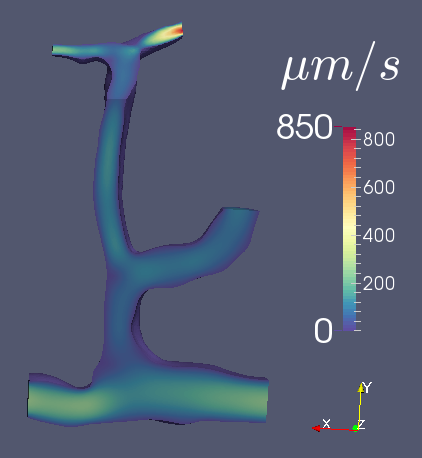
\includegraphics[scale=0.5]{vel_prof.png}
  \end{center}
  \caption{Velocity profile obtained from running the code from the implementation section, here viewed in ParaView. .}
 \label{fig:velocity_profile}
\end{figure}


\section{Squeezing a postdoc's brain}

We would very much like to squeeze postdoc Erika Lindström's brain. Since she has refused to let us do this with our hands in her office, we must do this on a computer using her brain as our computational domain. The brain will be deformed as a result of the squeezing and to capture this effect we will use a \emph{linear elastic} model. 

A mesh of Erika's brain can be found in the git repository. 

The brain is not clamped in the skull, but in a sense floating around. This means that we must employ \emph{neumann boundary conditions} on the entire boundary. As we know, there are no unique solution to such a problem since all \emph{rigid motions} satify the equation. So in order to obtain a unique solution we must remove all rigid motions. All the possible rigid motions in 3D are: translations in $x,y,z$-direction and rotations around the corresponding axes. Thus six in total.

An example using \emph{FEniCS} on how to remove these can be found in the same repository as the brain mesh. 

\subsection{Paraview}
\emph{ParaView} is an great open-source, multi-platform data analysis and visualization software. For instance results and other data generated using \emph{FEniCS} can be studied in more detial with ParaView.  

\subsubsection{Load/save state}

Being able to save your work and later properly load it is important. This is done using the \emph{save/load state} function in ParaView. If you are switching between computers, or collaborating with others, you might get some errors loading state files. This is because the state file uses the path to \texttt{.pvd}-file on which is was originally built, and that path is usually different on different computers.

\textbf{Example}: 
Let's try to open the state file \texttt{screen\_shot.pvsm} from where Figure [] is taken. ParaView will likely give you an error. To fix this open the file in a text editor, search for the name of the \texttt{.pvd}-file and you will fine one or more lines like:

\texttt{<Element index="0"value="/home/krister/..../deformed\_brain.pvd"/>}

Correct the path and load the state file in ParaView.


\subsection{Mathematical formulation}

Find $u$ such that 
\begin{align*}
  \int_\Omega  2\mu (\epsilon(u) : \epsilon(v))  +\lambda (\nabla \cdot u) (\nabla \cdot v) \: dx = \int_\Omega f \cdot v \: dx \quad \forall v \in V
\end{align*} 

Boundary conditions
\begin{align*}
\sigma \cdot \mathbf{n} = p\mathbf{n} \quad &on \quad \partial \Omega
\end{align*}

The material parameters for Erika's brain are $E = 16000 $ Pa and $\nu = 0.25$. The Lamè coefficients can be computed according to 
\begin{align*}
\lambda = \frac{E \nu}{(1-2\nu)(1+\nu)} \quad and \quad \mu = \frac{E}{2(1+\nu)}.
\end{align*}

\subsection{Implementation}

\begin{python}
from fenics import *

[Elasticity code to be included here]

\end{python}

\subsection{Results}

 \begin{figure}[h!] 
\begin{center}
  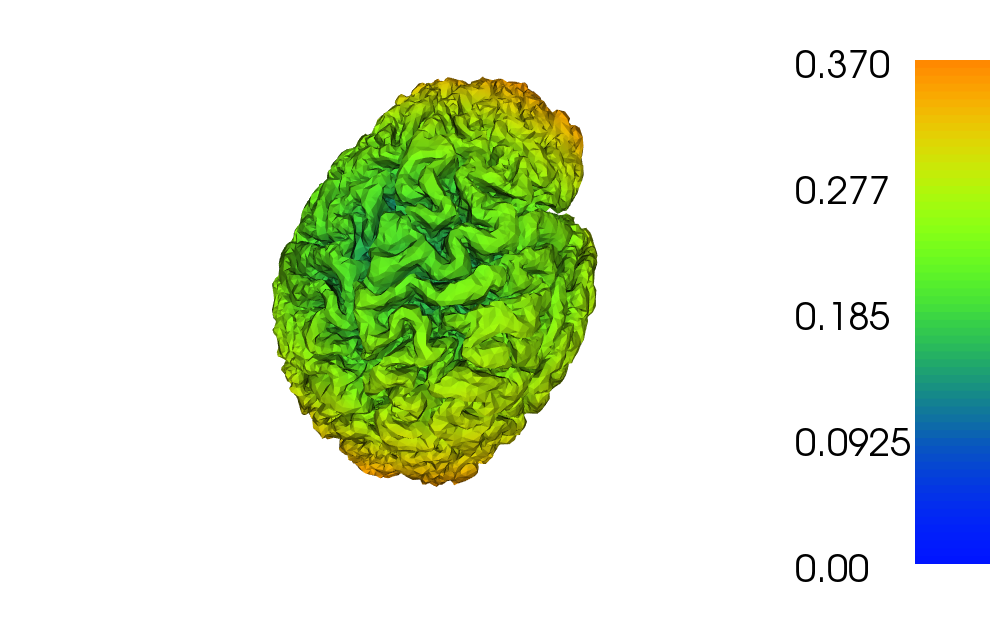
\includegraphics[scale=0.4]{brain.png}
  \end{center}
  \caption{Numerical solution using FEniCS. Displacement measured in $mm$.}
\end{figure}

\bibliographystyle{plain}
\bibliography{./papers}


\end{document}
